\chapter{Formalna verifikacija modela}
\label{ch:verif}

Ispravnost protokola može se provjeriti formalnom verifikacijom modela protokola
uz zadane preduvjete koje model
mora zadovoljiti. Protokol ACAP je specificiran i formalno verificiran s pomoću
alata Scyther~\cite{cremers2007scyther}. Scyther omogućuje formalnu verifikaciju
modela protokola i sigurnosnih zahtjeva uz korištenje sigurnosnih
primitiva poput sažetaka, simetrične kriptografije i kriptografije javnog ključa.

\comment{dodati kratko poglavlje o načinu na koji scyther verificira protokole}

U ovom poglavlju pojašnjena je sintaksa za specifikaciju modela protokola i
specificiran je model protokola ACAP. U nastavku se prikazuje izvođenje
definiranog modela i analiziraju se rezultati verifikacije.

\section{Značajke jezika SPDL}

Alat Scyther za opis protokola koristi jezik SPDL (\emph{Security Protocol Definition
Language}). U tom jeziku moguće je koristiti sljedeće pojmove:
\begin{itemize}
\item Kriptografske funkcije za standardne kriptografske operacije:
    \begin{itemize}
	\item kriptografski sažetak (\texttt{hashfunction}), 
	\item simetrično šifriranje podataka (\texttt{\{secret\}key})
	\item asimetrično šifriranje podataka (\texttt{\{secret\}pk\{I\}} ili
	    \texttt{\{hash\}sk\{I\}}).
    \end{itemize}
\item Korisnički definirane konstante za definiciju jednosmjernih funkcija
    (\texttt{Function}), jedinstvenih privremenih vrijednosti
    (\texttt{Nonce}) i univerzalnih varijabli (\texttt{Ticket}).
\item Definiciju protokola (\texttt{protocol ime\_protokola}) koja obuhvaća
    uloge (\texttt{role}) komunicirajućih strana. U svakoj
    ulozi definiraju se varijable koje se koriste za komunikaciju zajedno s
    događajima slanja (\texttt{send}) i primanja (\texttt{recv}) poruka koji
    opisuju komunikaciju. Nakon opisa komunikacije slijede definicije
    sigurnosnih zahtjeva na protokol (\texttt{claim}) koje se provjeravaju
    prilikom verifikacije.
\end{itemize}

U idućem poglavlju dan je primjer formalne verifikacije jednostavnog protokola
za uzajamnu autentifikaciju.

\section{Primjer verifikacije jednostavnog protokola}

Za primjer modeliranja i verifikacije jednostavnog protokola odabran je protokol
Needham-Schroeder-Lowe (NSL)~\cite{lowe1996breaking}. Protokol NSL je popravljena
inačica Needham-Schroeder protokola čija je osnovna namjena uzajamna
autentifikacija dvije komunicirajuće strane. Razmjena poruka u protokolu NSL
prikazana je izrazima na slici \ref{fig:nsl_spec}, gdje I predstavlja započinjatelja
(engl. \emph{initiatior}), a R primatelja (engl. \emph{responder}),
$N_X$ su \emph{nonce} vrijednosti, $PK_X$ javni ključevi, dok su uloge $I$ i $R$
identiteti komunicirajućih strana (certifikati ili javni ključevi).

\begin{figure}[htb]
    \begin{center}
\begin{tabular}{p{1.5cm} p{3.0cm}}
    I $\rightarrow$ R: & $(I, N_I)_{PK_R}$\\
    R $\rightarrow$ I: & $(N_I,N_R,R)_{PK_I}$\\
    I $\rightarrow$ R: & $(N_R)_{PK_R}$\\
\end{tabular}
    \end{center}
\vspace{-15pt}
\caption{Opis protokola Needham-Schroeder-Lowe}
\label{fig:nsl_spec}
\end{figure}

U modelu protokola definiraju se dvije uloge: započinjatelj I i primatelj R.
Definicija dvije osnovne uloge protokola NSL prikazana je na slici
\ref{fig:nsl_def}. Uloga \texttt{I} predstavlja klijenta, odnosno započinjatelja
komunikacije (engl. \emph{initiator}), a uloga \texttt{R} predstavlja
poslužitelja, odnosno primatelja (engl. \emph{responder}).

\begin{figure}[htb]
\begin{subfigure}[t]{0.5\linewidth}
\begin{small}
\begin{verbatim}
protocol nsl(I, R) {

  # uloga započinjatelja
  role I { ... }

  # uloga primatelja
  role R { ... }
}
\end{verbatim}
\end{small}
\vspace{-5pt}
\subcaption{Definicija uloga}
\label{fig:nsl_def}
\end{subfigure}
\begin{subfigure}[t]{0.5\linewidth}
\begin{small}
\begin{verbatim}
 role I {
  fresh ni: Nonce; var nr: Nonce;

  send_1(I,R, {I,ni}pk(R));
  recv_2(R,I, {ni,nr,R}pk(I));
  send_3(I,R, {nr}pk(R));
  ...
 }
\end{verbatim}
\end{small}
\vspace{-5pt}
\subcaption{Definicija varijabli i razmjene za ulogu I}
\label{fig:nsl_var_sr}
\end{subfigure}
\label{fig:nsl}
\vspace{-5pt}
\caption{Definicija protokola NSL}
\end{figure}

Na početku definicije svake uloge nalazi se definicija varijabli nužnih za
pojedinu ulogu. Ulogama u primjeru potrebne su samo varijable za \emph{nonce}
vrijednosti. Kod definicije varijabli važno je
napomenuti da li ta uloga stvara vrijednost ili zaprima vrijednost kroz razmjenu
poruka. Kod uloge koja stvara vrijednost navodi se ključna riječ \texttt{fresh},
a kod uloge koja zaprima vrijednost navodi se ključna riječ \texttt{var}.
Deklaracija varijabli za ulogu započinjatelja komunikacije
prikazana je na slici \ref{fig:nsl_var_sr}.

Uz deklaraciju varijabli na slici \ref{fig:nsl_var_sr} prikazana je i razmjena
poruka u protokolu NSL. Razmjena poruka u jeziku SPDL definira se događajima
\texttt{send} i \texttt{recv}. U sklopu tih događaja specificira se
pošiljatelj, primatelj i sadržaj poruke na sljedeći način:
\begin{itemize}
    \item slanje poruke: \texttt{send\_n(pošiljatelj, primatelj, sadržaj)},
    \item primanje poruke: \texttt{recv\_n(pošiljatelj, primatelj, sadržaj)},
\end{itemize}
pri čemu \texttt{n} identificira te događaje i služi za njihovo grupiranje.
Za svaki događaj slanja poruke u jednoj ulozi,
u jednoj od preostalih uloga
mora biti definiran odgovarajući
događaj primanja poruke. U suprotnom slučaju
formalna definicija protokola nije valjana.

Formalna definicija razmjene poruka za protokol NSL na slici
\ref{fig:nsl_var_sr} proizlazi iz opisa protokola na slici
\ref{fig:nsl_spec}.
Posljednji dio u definiciji uloge sadrži uvjete koje formalno modelirani
protokol mora zadovoljavati. Protokol NSL prema definiciji mora zadovoljavati
sljedeće zahtjeve:
\begin{itemize}
    \item Tajnost parametara \emph{nonce}, $N_I$ i $N_R$. U jeziku SPDL to se
	definira s ključnom riječi \texttt{Secret} koja kao argument prima
	parametar čija se tajnost ispituje.
    \item Da su svi događaji definirani unutar uloge uspješno završili.
	Definira se s ključnom riječi
	\texttt{Niagree} koja proizlazi iz izraza \emph{Non-injective agreement}
	\cite{scyther_book}.
    \item Da se događaji slanja unutar jedne uloge moraju izvršiti prije
	odgovarajućeg događaja primanja unutar druge uloge. Time se označava da
	napadač nije u mogućnosti poslati poruku koja bi na neki način
	poremetila razmjenu. Definira se s ključnom riječi \texttt{Nisynch} koja
	označava pojam \emph{Non-injective synchronization} \cite{scyther_book}.
\end{itemize}

Zadovoljavanje određenih zahtjeva definira se s ključnom riječi \texttt{claim}.
Uz ključnu riječ navodi se uloga u kojoj zahtjev mora biti zadovoljen,
definicija zahtjeva i parametar ako je potreban. Formalna definicija zahtjeva za
ulogu započinjatelja I prikazana je na slici \ref{fig:nsl_claims}.

\begin{figure}[htb]
    \centering
\begin{small}
\begin{BVerbatim}
 role I {
  ...
  claim_i1(I,Secret,ni);
  claim_i2(I,Secret,nr);
  claim_i3(I,Niagree);
  claim_i4(I,Nisynch);
 }
\end{BVerbatim}
\end{small}
\vspace{-5pt}
\caption{Definicija zahtjeva za ulogu I protokola NSL}
\label{fig:nsl_claims}
\end{figure}

Cjelokupan model za protokol NSL prikazan je na slici \ref{fig:nsl_def_full} i u
njemu vidljive su razlike između definicija varijabli te događaja primanja
i slanja poruka između uloga započinjatelja I i primatelja R.

Potpuni formalni model protokola provjerava se pomoću alata Scyther i opcije
\emph{characterize}, koja dani model pokreće i provjerava jesu li definirane
uloge uspješno završile definirane događaje slanja i primanja. Potom slijedi
formalna verifikacija specificiranih uvjeta za modelirani protokol. Rezultat
provjere i formalne verifikacije specificiranog modela prikazan je na slici
\ref{fig:nsl_char}. Dijagram toka za protokol NSL prikazan je na slici
\ref{fig:char_nsl}.

\begin{figure}[H]
    \begin{subfigure}{0.58\textwidth}
\begin{small}
\begin{verbatim}
protocol nsl(I,R) {
 role I {
  fresh ni: Nonce; var nr: Nonce;

  send_1(I,R,{I,ni}pk(R));
  recv_2(R,I,{ni,nr,R}pk(I));
  send_3(I,R,{nr}pk(R));

  claim_i1(I,Secret,ni); claim_i2(I,Secret,nr);
  claim_i3(I,Niagree); claim_i4(I,Nisynch);
 }
 role R {
  var ni: Nonce; fresh nr: Nonce;

  recv_1(I,R,{I,ni}pk(R));
  send_2(R,I,{ni,nr,R}pk(I));
  recv_3(I,R,{nr}pk(R));

  claim_r1(R,Secret,ni); claim_r2(R,Secret,nr);
  claim_r3(R,Niagree); claim_r4(R,Nisynch);
 }
}
\end{verbatim}
\end{small}
\caption{SPDL model protokola NSL}
\label{fig:nsl_def_full}
\end{subfigure}
\begin{subfigure}{0.428\textwidth}
\begin{centering}
    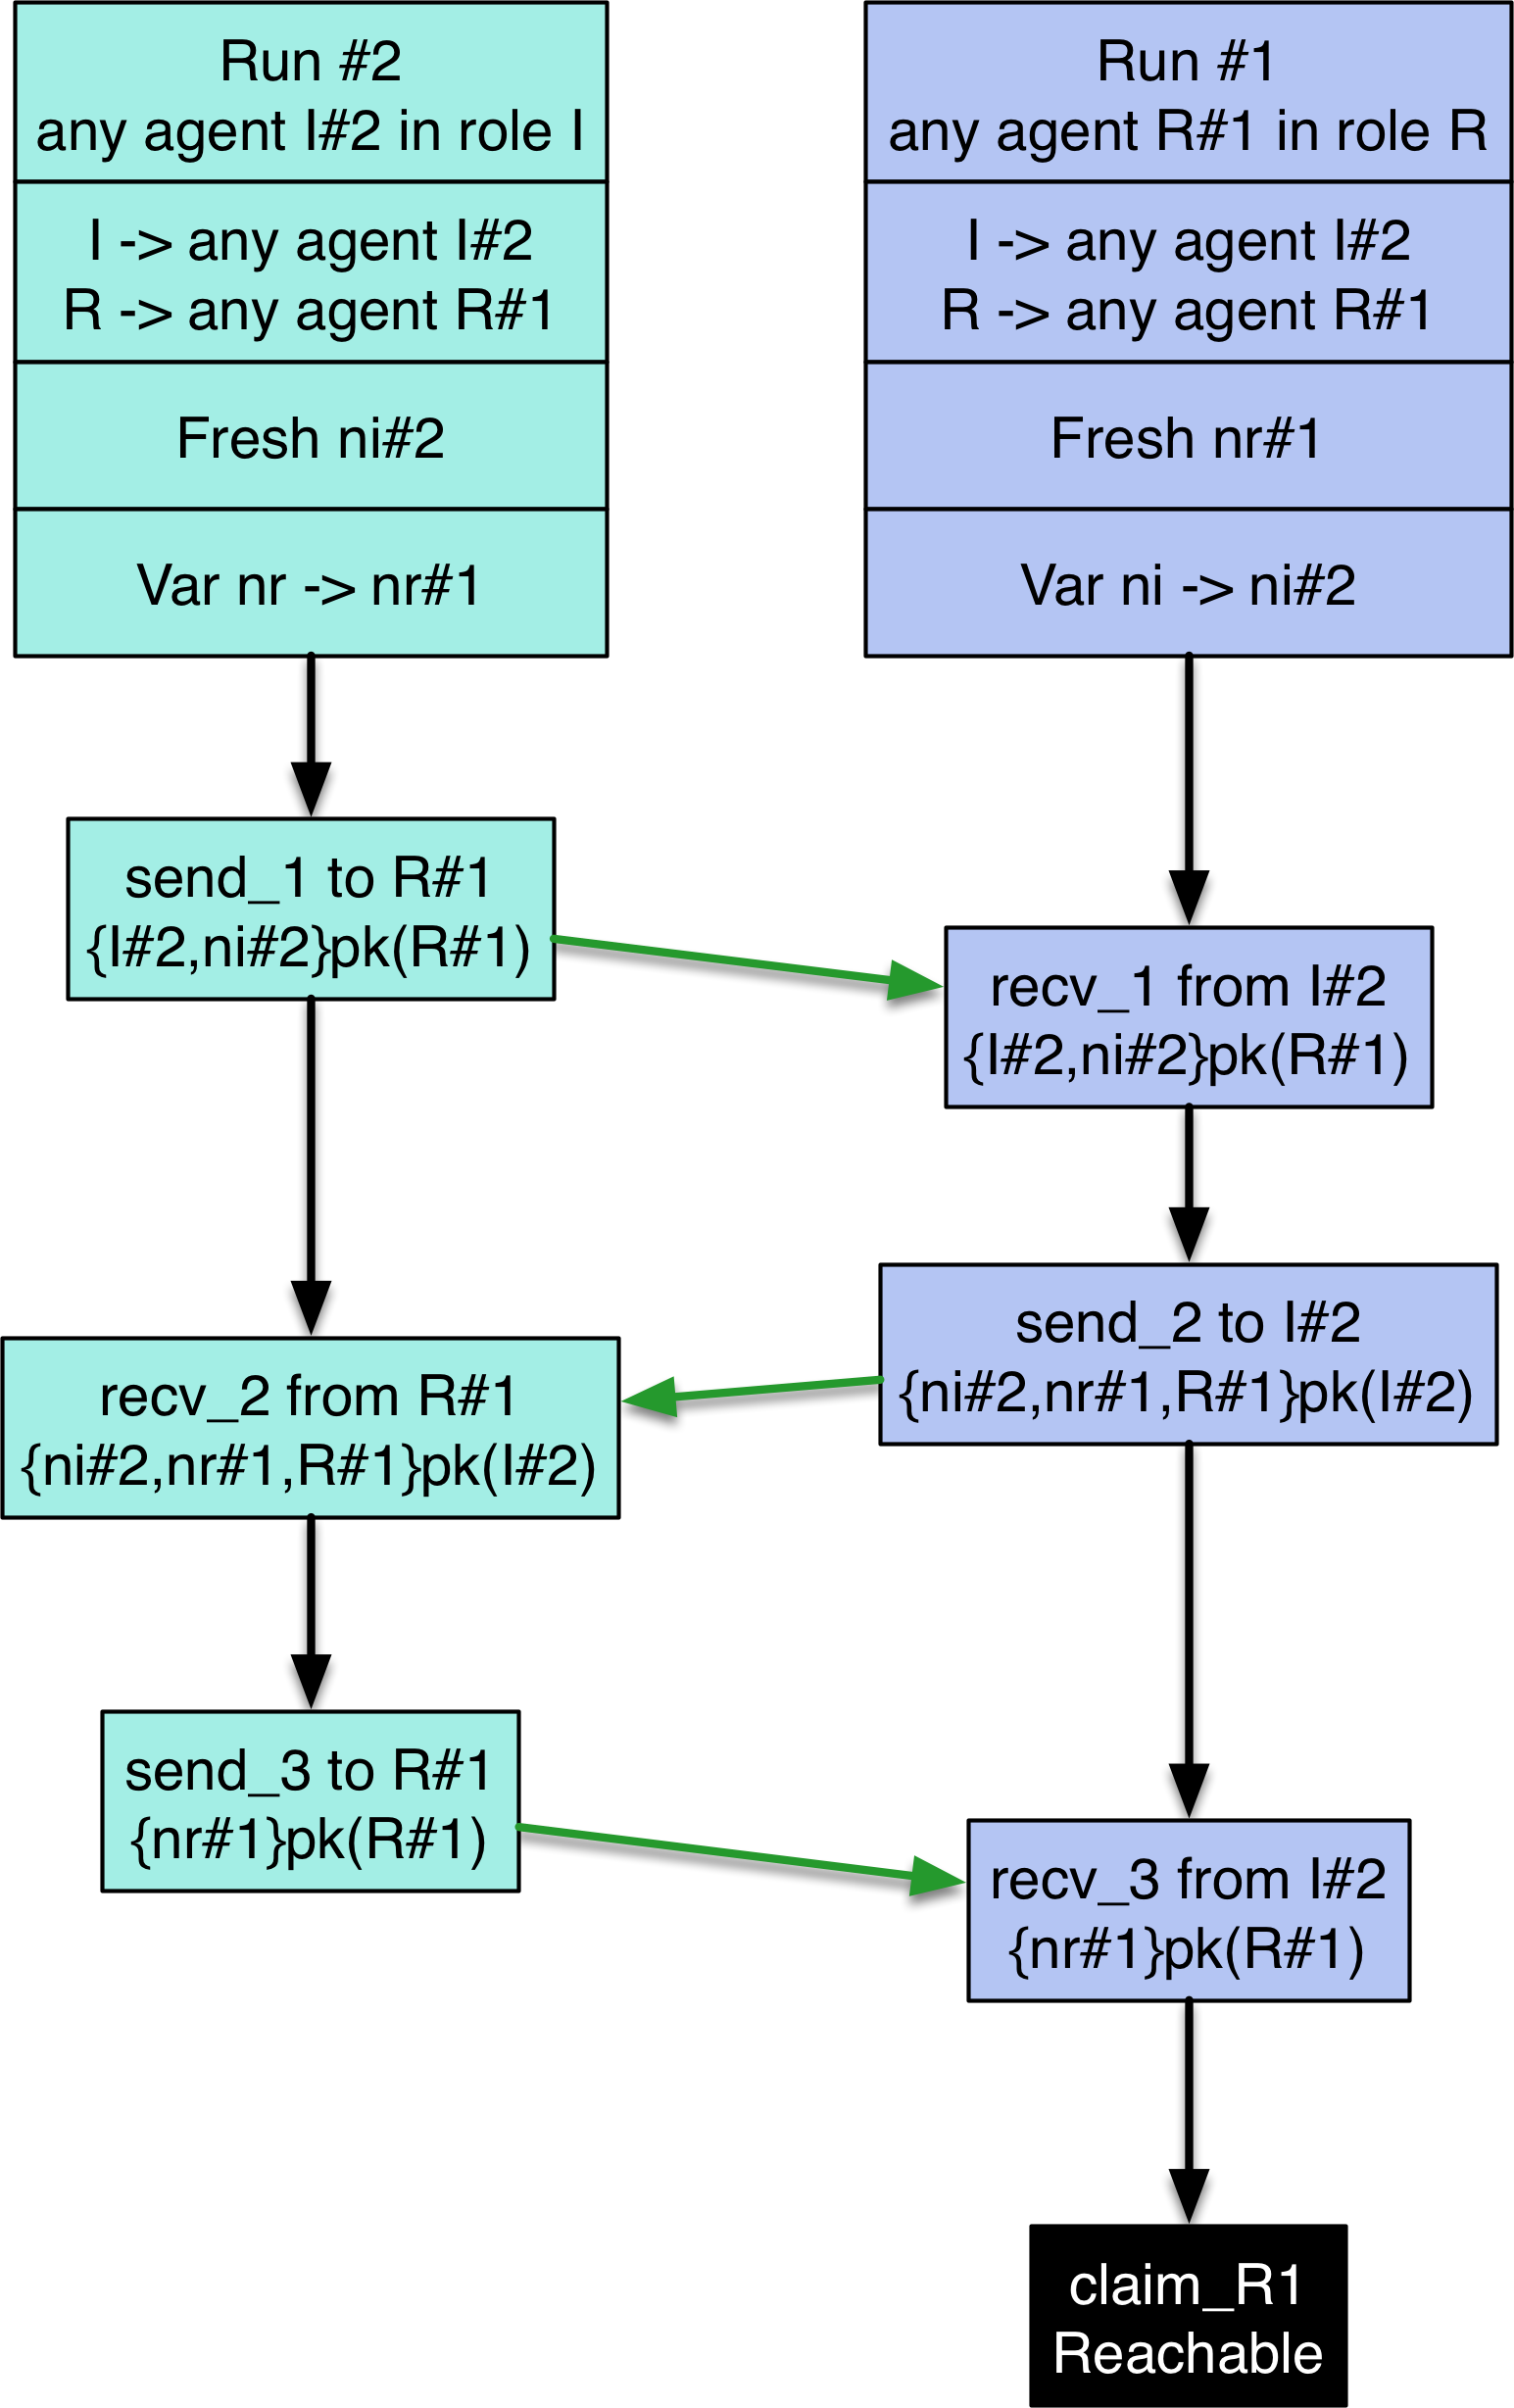
\includegraphics[width=0.95\textwidth]{unt2.png}
    \vspace{9pt}
    \caption{Dijagram toka za protokol NSL}
    \label{fig:char_nsl}
\end{centering}
\end{subfigure}
\caption{SPDL model i dijagram toka za protokol Needham-Schroeder-Lowe}
\end{figure}

\begin{figure}[htb]
\begin{framed}
\begin{small}
\begin{verbatim}
$ scyther-linux -c nsl.spdl 
claim   nsl,I   Reachable_I1    -       Ok      [exactly 1 variant]
claim   nsl,R   Reachable_R1    -       Ok      [exactly 1 variant]
$ scyther-linux nsl.spdl 
claim   nsl,I   Secret_i1       ni      Ok      [proof of correctness]
claim   nsl,I   Secret_i2       nr      Ok      [proof of correctness]
claim   nsl,I   Niagree_i3      -       Ok      [proof of correctness]
claim   nsl,I   Nisynch_i4      -       Ok      [proof of correctness]
claim   nsl,R   Secret_r1       ni      Ok      [proof of correctness]
claim   nsl,R   Secret_r2       nr      Ok      [proof of correctness]
claim   nsl,R   Niagree_r3      -       Ok      [proof of correctness]
claim   nsl,R   Nisynch_r4      -       Ok      [proof of correctness]
\end{verbatim}
\end{small}
\vspace{-15pt}
\end{framed}
\caption{Rezultati provjere i verifikacije modela protokola NSL}
\label{fig:nsl_char}
\end{figure}

\begin{figure}[H]
\end{figure}


\section{Model predloženog protokola ACAP}

Opis protokola ACAP korištenjem SPDL-a sastoji se od glavnog protokola
(\texttt{protocol acap\{I, R\}}) i pomoćnog protokola (\texttt{protocol
@executability \{DH, O\}}), koji se koristi za operacije vezane uz
Diffie-Hellman razmjenu ključeva.

Glavni protokol ACAP sastoji se od dvije glavne uloge \texttt{I} i \texttt{R}
isto kao i protokol Needham-Schreoder-Lowe. U sklopu uloga definiraju se
varijable koje su specifične za protokol ACAP.

Svakoj ulozi potreban je sljedeći niz varijabli:
\begin{itemize}
    \item eksponent za Diffie-Hellman dogovor ključeva,
    \item nasumične vrijednosti za jednokratno korištenje (engl. \emph{nonce})
	za obje strane,
    \item univerzalna varijabla za zaprimanje javnog dijela Diffie-Hellman
	razmjene,
    \item dvije varijable koje sadrže popise algoritama.
\end{itemize}
Deklaracije varijabli za obje uloge prikazane su na slici \ref{fig:var_def}. 

\begin{figure}[htb]
\begin{small}
\begin{verbatim}
protocol acap(I,R) {
  role I {
    # stvaranje novog DH eksponenta i noncea
    fresh i, Ni: Nonce;
    # varijabla za zaprimanje noncea
    var Nr: Nonce;
    # varijabla za zaprimanje javnog dijela DH razmjene
    var Gr: Ticket;
    # stvaranje novog popisa algoritama
    fresh Li: AlgList;
    # varijabla za zaprimanje popisa algoritama
    var Lr: AlgList;
    ...
  }
  role R {
    fresh r, Nr: Nonce; var Ni: Nonce;
    var Gi: Ticket;
    fresh Lr: AlgList; var Li: AlgList;
    ...
  }
}
\end{verbatim}
\end{small}
\vspace{-15pt}
\caption{Prikaz varijabli za uloge započinjatelja i primatelja}
\label{fig:var_def}
\end{figure}

Nakon definicije varijabli i njihovog stvaranja slijedi tijek razmjene poruka
između komunicirajućih strana. Da bi dvije uloge unutar protokola uspješno
razmijenile poruke nužno je da svaki događaj slanja poruke ima odgovarajući
događaj primanja poruke s druge strane. Na slici \ref{fig:i_msgs} prikazani su
događaji slanja i primanja na strani započinjatelja dok je na slici
\ref{fig:r_msgs} prikazano isto za ulogu primatelja.

\begin{figure}[htb]
\begin{small}
\begin{verbatim}
  role I {
    ...
    send_1( I, R, g(i), Ni);
    recv_!2( R, I, Gr, Nr, R, {h(Gr)}sk(R), MAC(h(Gr,i), R, Ni, Nr) );
    send_!3( I, R, I, Li, {h(Li, g(i), Gr)}sk(I), MAC(h(Gr,i), I) );
    recv_4( R, I, Lr, {h(g(i), Gr, Lr)}sk(R) );
    ...
  }
\end{verbatim}
\end{small}
\vspace{-15pt}
\caption{Komunikacija sa strane započinjatelja}
\label{fig:i_msgs}
\end{figure}

\begin{figure}[htb]
\begin{small}
\begin{verbatim}
  role R {
    ...
    recv_1( I, R, Gi, Ni);
    send_!2( R, I, g(r), Nr, R, {h(g(r))}sk(R), MAC(h(Gi,r), R, Ni, Nr) );
    recv_!3( I, R, I, Li, {h(Li, Gi, g(r))}sk(I), MAC(h(Gi,r), I) );
    send_4( R, I, Lr, {h(Gi, g(r), Lr)}sk(R) );
    ...
  }
\end{verbatim}
\end{small}
\vspace{-15pt}
\caption{Komunikacija sa strane primatelja}
\label{fig:r_msgs}
\end{figure}

Prvi događaj slanja (\texttt{send\_1( I, R, g(i), Ni);}) ide od uloge \texttt{I}
prema ulozi \texttt{R} i sadrži parametre definirane za poruku \initi{}.
Odgovarajući događaj
primanja (\texttt{recv\_1( I, R, Gi, Ni);}) definira da poruka dolazi od uloge
\texttt{I}, a prima ju uloga \texttt{R}. Ovakav način pozivanja označava
komunikaciju između uloga \texttt{I} i \texttt{R}.
    
U danom je primjeru vidljivo da događaj \texttt{send\_1} odgovara događaju
\texttt{recv\_1} uz jednakost izraza \texttt{g(i)} i \texttt{Gi}. Isto vrijedi i
za izraze \texttt{send\_4} i \texttt{recv\_4} ako se u obzir uzme i jednakost
\texttt{g(r)} i \texttt{Gr}. Navedene jednakosti su potrebne kako bi
komunicirajuće strane mogle izvesti potrebne operacije.

U modelu je potrebno specificirati i zasebnu ulogu koja će omogućiti razmjenu
poruka definiranu događajima \texttt{send\_!2} i \texttt{recv\_!2} te
\texttt{send\_!3} i \texttt{recv\_!3} koji izravno ne odgovaraju jedan drugome.
Ti događaji uključuju poseban znak \texttt{!} (uskličnik), koji specificira da se
poruka šalje svim ulogama koje su dostupne u sklopu procesa verifikacije, a ne
samo između definiranih primatelja i pošiljatelja. Uloge u procesu verifikacije
obuhvaćaju sve definirane uloge, uključujući i ulogu napadača.
U sljedećem potpoglavlju dan je opis dodatnog protokola za modeliranje
Diffie-Hellman operacija.

\subsection{Modeliranje Diffie-Hellman operacija}

U alatu Scyther v1.1.3, koja je bila dostupna za vrijeme pisanja
disertacije nije podržano izravno korištenje Diffie-Hellman operacija.
Stoga je potrebno napraviti apstrakciju s pomoću integriranih operacija.
Diffie-Hellman (DH) operacije izračunavanja zamijenjene su jednosmjernom
funkcijom. DH operacija definirana izrazom $A = g^a mod p$ zamijenjena je
funkcijom g (\texttt{hashfunction g}) i izrazom \texttt{g(a)}, zbog pretpostavke
da operacija nije
reverzibilna, što vrijedi za tu vrstu potenciranja i računanja ostatka kao i za
funkciju sažetka unutar alata Scyther. Zbog tog svojstva primatelj podataka
poslanu informaciju \texttt{g(i)} prima pomoću univerzalne varijable
\texttt{Ticket Gi}.

Drugi dio DH izračuna odrađuje se s pomoću funkcije sažetka h
(\texttt{hashfunction h}) i rezultat te operacije je zajednička tajna u sklopu
DH razmjene. Izraz $S = (g^a mod p)^b$ istovjetan je izrazu \texttt{h(g(a),b)}.
Potrebno je i definirati da je operacija komutativna kako bi eventualni napadač uz
poznavanje jednog tajnog dijela DH razmjene (\texttt{a} ili \texttt{b}) mogao
doći do razmijenjene tajne. To je izvedeno s pomoću uloge \texttt{DH} u pomoćnom
protokolu (\texttt{@executability}) kojim se postiže jednakost \texttt{h(g(r),i)
= h(g(i),r)}, kako je prikazano na slici \ref{fig:exec_dh}. U toj specifikaciji je
korišten simbol uskličnika kod slanja i primanja kako bi ta jednakost vrijedila
za sve definirane uloge i napadača.

\begin{figure}[htb]
\begin{small}
\begin{verbatim}
protocol @executability (DH, O) {
  role DH {
    # definicija DH eksponenata
    var i, r: Nonce;
    # primi od bilo kojeg pošiljatelja
    recv_!DH1( DH, DH, h(g(r),i) );
    # pošalji bilo kojem primatelju ekvivalentni izraz
    send_!DH2( DH, DH, h(g(i),r) );
  }
  role O { ... }
}
\end{verbatim}
\end{small}
\vspace{-22pt}
\caption{Komutativnost Diffie-Hellman operacije}
\label{fig:exec_dh}
\end{figure}

Pomoćni protokol sadrži još jednu ulogu \texttt{O} koja se koristi za uspješnu
razmjenu poruka \initr{} i \listi{}, koje koriste zajedničku tajnu uspostavljenu
kroz DH za stvaranje zaštitnog HMAC sažetka. Uloga \texttt{O}
prikazana je na slici \ref{fig:exec_o}. Razmjena poruka između uloga \texttt{I}
i \texttt{R} odvija se kroz tu ulogu. Na slici su prikazani događaji
\texttt{send} i \texttt{recv} koji su povezani tom ulogom.

\begin{figure}[H]
\begin{small}
\begin{verbatim}
role O {
  var i, r, Ni, Nr: Nonce;
  var I, R: Agent; var Li: AlgList;
  ### razmjena poruke INITr (R->I) ###
  #send događaj u ulozi R
  #send_!2( R, I, g(r), Nr, R, {h(g(r))}sk(R), MAC(h(  Gi,r), R, Ni, Nr) );
  recv_!01( O, O, g(r), Nr, R, {h(g(r))}sk(R), MAC(h(g(i),r), R, Ni, Nr) );
  send_!02( O, O, g(r), Nr, R, {h(g(r))}sk(R), MAC(h(g(r),i), R, Ni, Nr) );
  #recv događaj u ulozi I
  #recv_!2( R, I,   Gr, Nr, R, {h(  Gr)}sk(R), MAC(h(  Gr,i), R, Ni, Nr) );
  ### razmjena poruke LISTi (I->R) ###
  #send događaj u ulozi I
  #send_!3( I, R, I, Li, {h(Li, g(i),   Gr)}sk(I), MAC(h(  Gr,i), I) );
  recv_!03( O, O, I, Li, {h(Li, g(i), g(r))}sk(I), MAC(h(g(r),i), I) );
  send_!04( O, O, I, Li, {h(Li, g(i), g(r))}sk(I), MAC(h(g(i),r), I) );
  #recv događaj u ulozi I
  #recv_!3( I, R, I, Li, {h(Li,   Gi, g(r))}sk(I), MAC(h(  Gi,r), I) );
}
\end{verbatim}
\end{small}
\vspace{-22pt}
\caption{Razmjena poruka \initr{} i \listi{} definirana u ulozi \texttt{O}}
\label{fig:exec_o}
\end{figure}

\section{Formalna verifikacija modela}
\label{sec:verif}
Prvi korak provjere ispravnosti modela je provjera
uspješnog završetka komunikacije s obje strane.
Alat Scyther nakon uspješne provjere generira dijagram toka za
specificirani model. Dijagram toka za model protokola ACAP prikazan je na slici
\ref{fig:characterize}. 

\begin{figure}[H]
\begin{centering}
    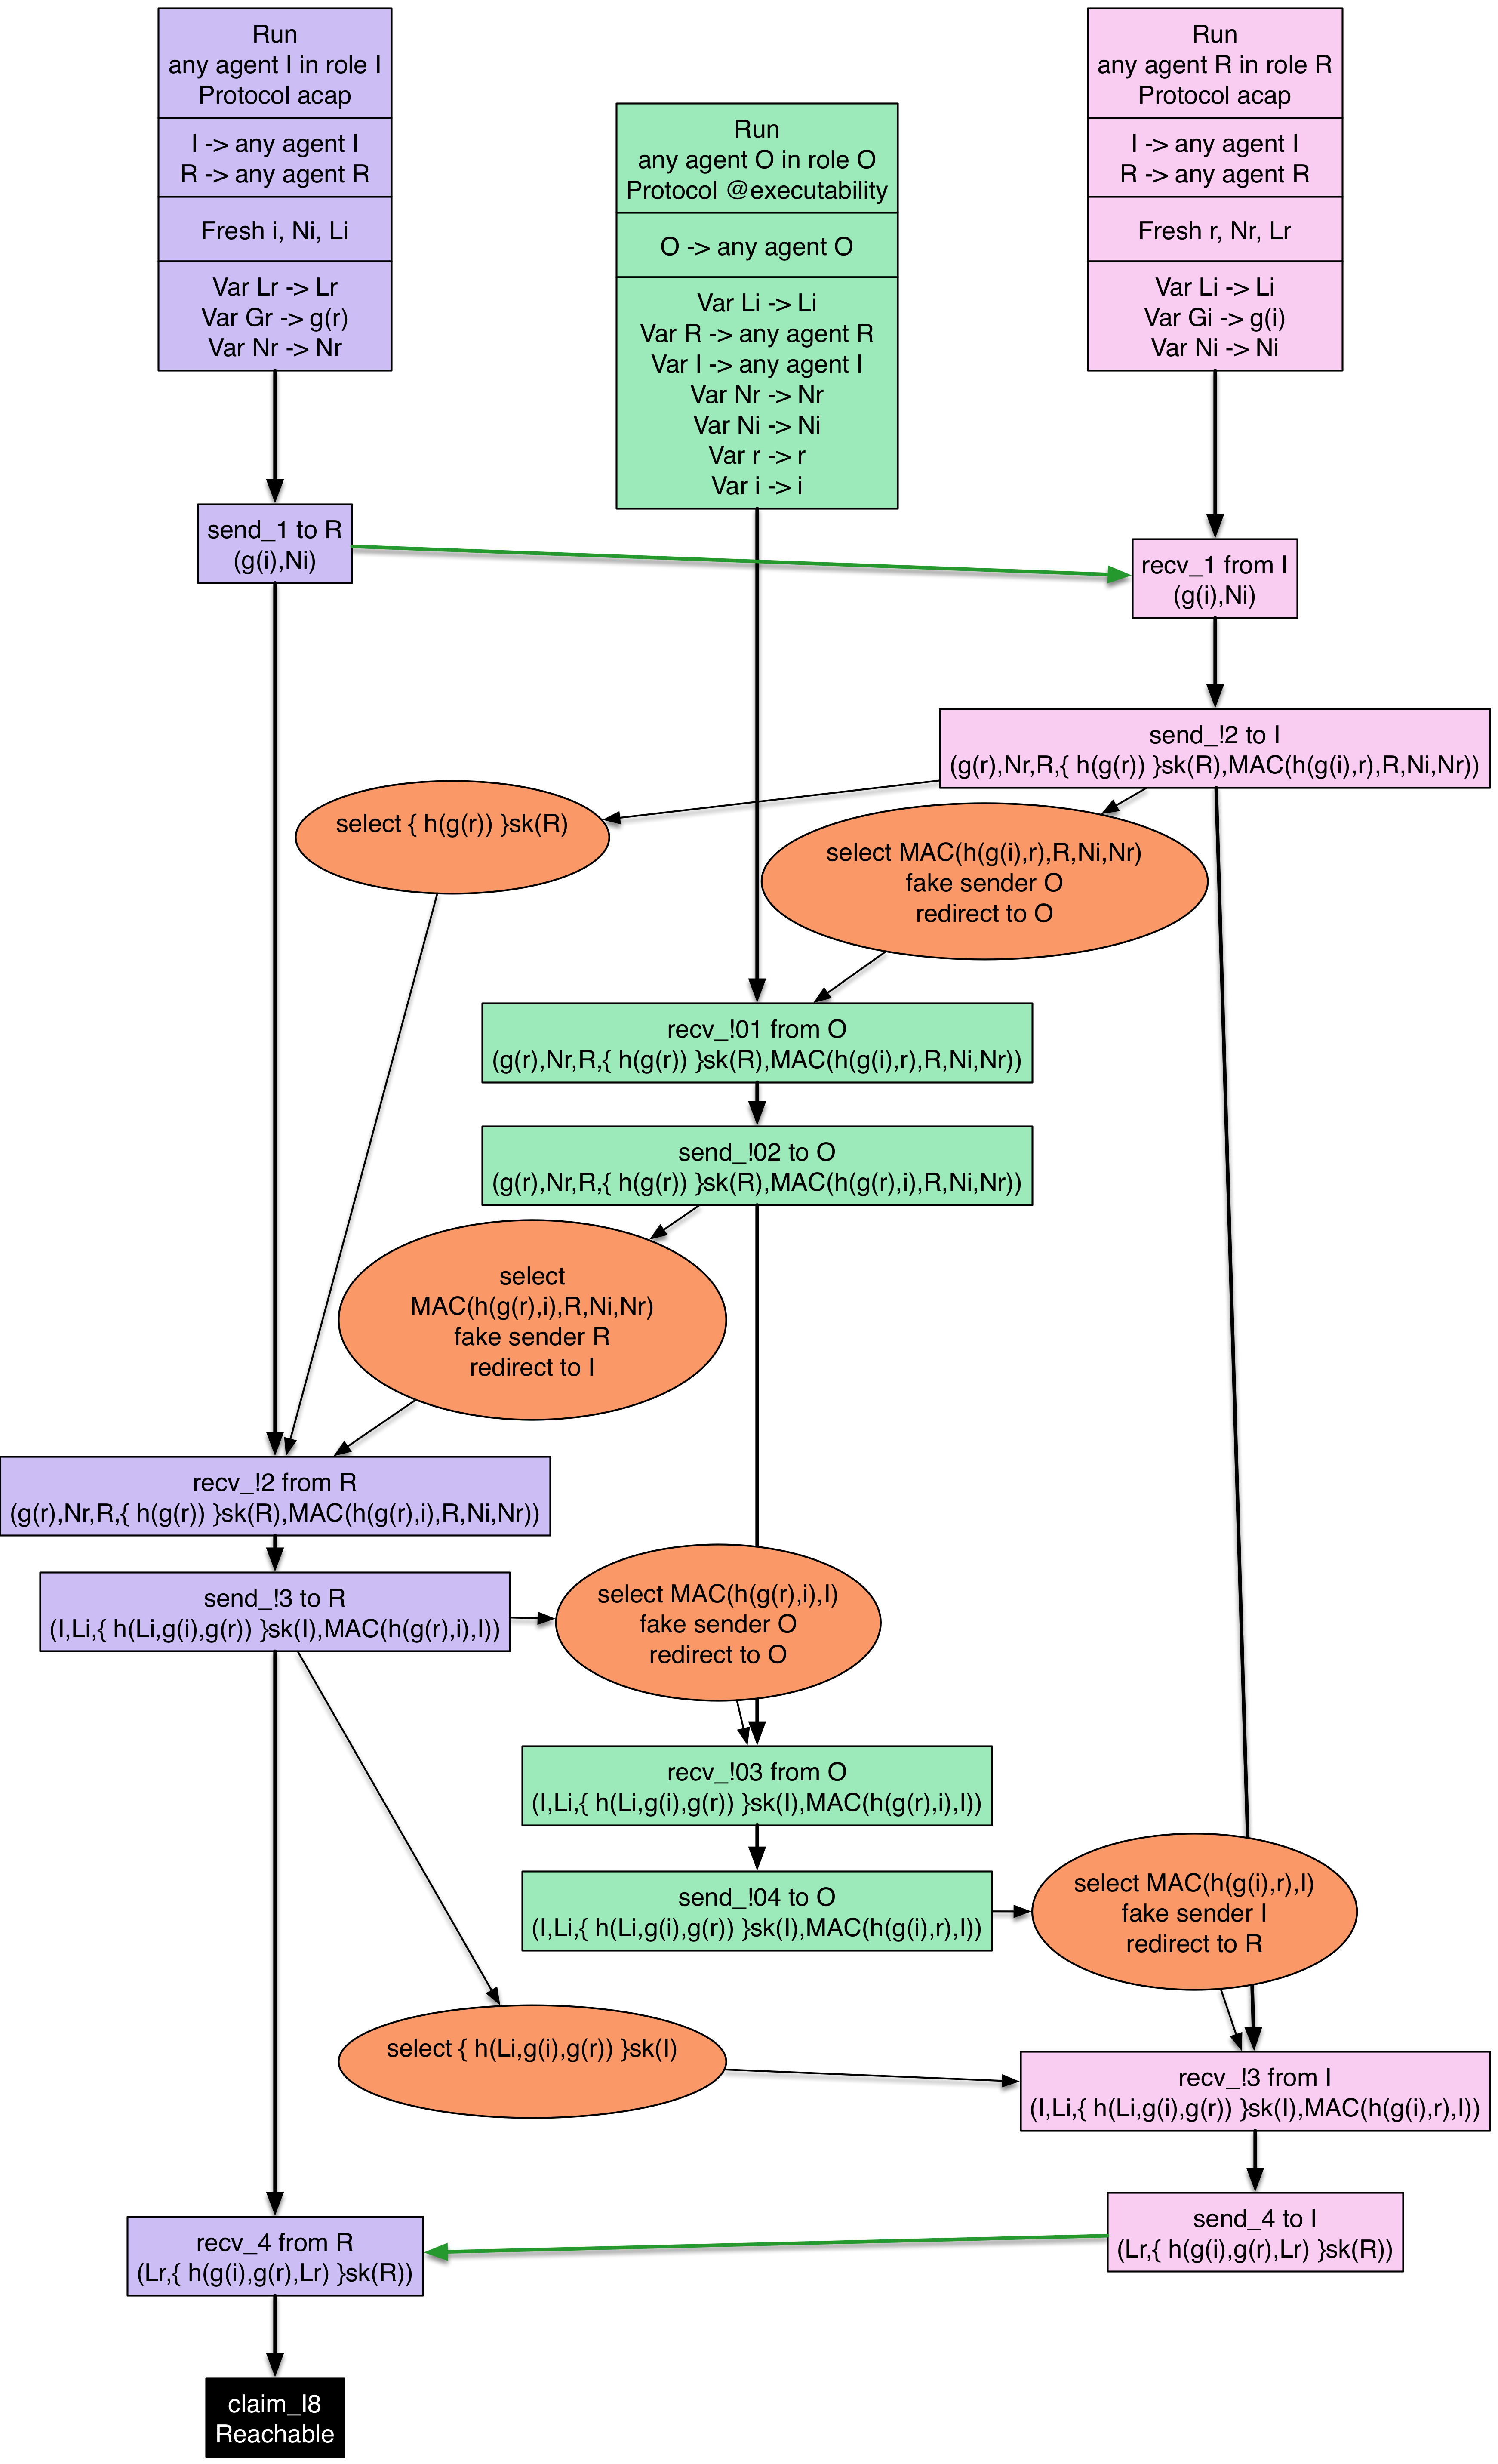
\includegraphics[width=0.75\textwidth]{graf}
    \caption{Dijagram toka za protokol ACAP}
    \label{fig:characterize}
\end{centering}
\end{figure}

Na slici se vidi da su za jednu uspješnu razmjenu
poruka potrebne tri uloge: uloga započinjatelja (\texttt{Role I}) i uloga
primatelja (\texttt{Role R}) u sklopu glavnog protokola i dodatna uloga za
upravljanje DH razmjenom (\texttt{Role O}) u sklopu pomoćnog protokola.

\subsection{Definicija sigurnosnih zahtjeva}

Nakon definiranja poruka i tijeka komunikacije, za svaku ulogu u modelu potrebno
je
odrediti sigurnosne zahtjeve koji trebaju biti zadovoljeni. Sigurnosni zahtjevi
za modelirani protokol su sljedeći:
\begin{itemize}
    \item Javni dijelovi DH razmjene moraju ostati nepromijenjeni za vrijeme
	razmjene kako bi obje strane imale istu zajedničku tajnu za vrijeme
	komunikacije. To se provjerava s pomoću sigurnosnog zahtjeva
	\texttt{claim} s ključnim riječima \texttt{Running} i \texttt{Commit}.
    \item Zajednička tajna ni u jednom trenutku tijekom razmjene ne smije doći do
	uloge napadača. Ta tvrdnja se provjerava koristeći ključnu riječ
	\texttt{SKR} (engl. \emph{Session Key Reveal}) koja označava otkrivanje ključa
	trenutne sjednice.
    \item Napadač ne smije imati nikakav utjecaj na razmjenu poruka, što
	predstavlja otpornost protokola na napade ponavljanja i napade s
	napadačem u sredini (\emph{man in the middle}). Sigurnosni zahtjev
	postavlja se s ključnom riječi \texttt{Nisynch} koja predstavlja pojam ne
	injektivne sinkronizacije (engl. \emph{Non-injective synchronization})
	\cite{scyther_book}.
\end{itemize}

Definirani sigurnosni zahtjevi prikazani su na slici \ref{fig:claims}.

\begin{figure}[htb]
\begin{small}
\begin{verbatim}
role R {
  recv_1( I, R, Gi, Ni);
  # početak praćenja javnih dijelova DH razmjene
  claim_R1( R, Running, I, g(r), Gi);
  send_!2( ... ); recv_!3( ... ); send_4( ... );

  # provjera istovjetnosti početnih i krajnjih vrijednosti
  claim_R2( R, Commit, I, g(r), Gi);
  # zahtjev tajnosti nad zajedničkom tajnom
  claim_R3( R, SKR, KDF(h(Gi,r)) );
  # zahtjev da napadač nije u mogućnosti utjecati na komunikaciju
  claim_R4( R, Nisynch );
}
\end{verbatim}
\end{small}
\vspace{-15pt}
\caption{Definicija sigurnosnih zahtjeva za modelirani protokol}
\label{fig:claims}
\end{figure}
\vspace{-10pt}

\subsection{Rezultati formalne verifikacije}

Verificirani model protokola ACAP nalazi se u dodatku \ref{app:model}.
Na adresi \url{http://public.tel.fer.hr/acap} nalazi se potpuni model i
rezultati verifikacije uz programsko ostvarenje i primjer izvođenja.
Prilikom pokretanja
verifikacije moguće je odrediti broj paralelnih uloga koje će se izvoditi u
pokušaju napada na protokol. Moguće je verificirati i uz neograničen broj
paralelnih uloga, što u potpunosti dokazuje istinitost definiranih sigurnosnih
zahtjeva. Model protokola ACAP verificiran je uz neograničen broj paralelnih
uloga kod testiranja i pokazano je da su svi definirani sigurnosni zahtjevi
zadovoljeni.  
Rezultati verifikacije s alatom Scyther prikazani su na slici
\ref{fig:verif_res}.
Zahtjevi \texttt{I2} i \texttt{R2} pokazuju da ne dolazi do promjene parametara
DH razmjene,
zahtjevi \texttt{I3} i \texttt{R3} pokazuju da zajednička tajna nije otkrivena,
a zahtjevi \texttt{I4} i \texttt{R4} da napadač ne može utjecati na razmjenu
poruka.

\begin{figure}[ht]
\begin{centering}
\begin{framed}
\begin{small}
\begin{verbatim}
$ scyther-linux acap.spdl
claim   acap,I  Commit_I2       (R,g(i),Gr)     Ok  [no attack within bounds]
claim   acap,I  SKR_I3  KDF(h(Gr,i))    Ok      [no attack within bounds]
claim   acap,I  Nisynch_I4      -       Ok      [no attack within bounds]
claim   acap,R  Commit_R2       (I,g(r),Gi)     Ok  [no attack within bounds]
claim   acap,R  SKR_R3  KDF(h(Gi,r))    Ok      [no attack within bounds]
claim   acap,R  Nisynch_R4      -       Ok      [no attack within bounds]
\end{verbatim}
\end{small}
\vspace{-15pt}
\end{framed}
\vspace{-15pt}
\caption{Rezultati verifikacije protokola s alatom Scyther}
\label{fig:verif_res}
\end{centering}
\end{figure}
\vspace{-10pt}

Proces formalne verifikacije posebno je zahtjevan zbog zasebnog modeliranja
Diffie-Hellman operacija koje prouzrokuju veći broj stanja za provjeru nego što
je potrebno. Zahtjevnost se očituje u količini vremena i resursa koji su
potrebni za verifikaciju protokola. Što je veći broj paralelnih uloga u
verifikaciji to verifikacija traje dulje i veći su zahtjevi na radnu memoriju
(RAM) u sustavu.
Formalna verifikacija izvodila se na 6 jezgara procesora Intel Xeon E5-2680
(frekvencije 2.70 Ghz) s 40 GB radne memorije. Trajanje verifikacije
prikazano je u tablici \ref{tab:verif_dur}. Verifikacija se izvodila paralelno
na svih 6 jezgara kako bi se skratilo vrijeme izvođenja verifikacije, ali to je
ujedno i povećalo zahtjeve za radnom memorijom.

\begin{table}[htb]
\caption{Trajanje formalne verifikacije ovisno o broju paralelnih uloga}
\renewcommand{\arraystretch}{1.25}
\label{tab:verif_dur}
\centering
\small
\begin{tabular}{ c  c }
\toprule
Broj uloga & Trajanje verifikacije (min)
    \\ \midrule
%    3 & 0.2
%    \\ \hline
    4 & 2.3 
    \\ \hline
    5 & 13.0
    \\ \hline
    6 & 52.0
    \\ \hline
    7 & 174.0
    \\ \hline
    8 & 457.0
    \\ \hline
    9 & 877.0
    \\ \hline
    10 & 1255.0
    \\ \hline
    neograničen & 1532.0
    \\ \bottomrule
\end{tabular}
\end{table}

Prema dobivenim vrijednostima trajanja verifikacije može se zaključiti kako se
povećavanjem broja uloga značajno povećava broj stanja koje je potrebno
provjeriti, što iziskuje veću količinu vremena. Može se primijetiti da su
zadnje dvije verifikacije slične po trajanju, što upućuje da je verifikacija s
10 uloga došla blizu maksimalnog broja stanja kojeg je moguće postići sa
specificiranim modelom protokola.


% vim: spell spelllang=hr
